\section{A szoftver architektúrája}

\subsection{Futási környezet}

A kliens program webes technológiákon alapul, így működtethető böngészőből,
illetve böngészőtől független önálló becsomagolt állományból is.

\subsection{Felhasznált főbb könyvtárak}

\begin{itemize}
  \item \textbf{Electron}: Az önlállóan futtatható becsomagolt állomány
  létrehozásához. \\
  https://electronjs.org/

  \item \textbf{Redux}: Az alkalmazás központi állapotának tárolásához és
  kezeléséhez. (A tradicionális MVC architektúrából leginkább a modell és a
  kontroller kombinációjának feleltethető meg.) \\
  https://redux.js.org/

  \item \textbf{Golden Layout}: A dinamius, felhasználó által személyre szabható
  felület kialakítására. \\
  https://golden-layout.com/

  \item \textbf{Material UI}: A felhasználói felületen megjelenő elemek
  kinézetéhez. \\
  http://www.material-ui.com/ | https://material-ui-next.com/

  \item \textbf{OpenLayers}: A térképes megjelenítéshez. \\
  https://openlayers.org/

  \item \textbf{React}: A központi állapot nézetté történő leképezésére, a HTML
  elemek fölött használt állapottal rendelkező komponensek absztrakciójának
  megteremtésére. (A hagyományos MVC architektúrában leginkább a view szerepét
  tölti be.) \\
  https://reactjs.org/

  \item \textbf{ol-react}: Az OpenLayers könyvtár által nyújtott funkciók React
  komponensekként való kezeléséhez. \\
  https://www.npmjs.com/package/ol-react

  \item \textbf{mini-signals}: Az alkalmazás komponensei közötti üzenetküldésre.
  \\
  https://github.com/Hypercubed/mini-signals
\end{itemize}

\subsection{A megvalósított osztályok}

\subsubsection{HeatmapLayerSettingsPresentation}
A hőtérkép réteg beállításait tartalmazó komponens.
Itt adhatóak meg az aktuális réteg úgymond "feliratkozásai", tehát, hogy melyik
eszköz melyik csatornáján érkező adatok megjelenítését végezze.
Beállítható továbbá a jelölők közötti távolság, hogy rácspontokon kerüljenek-e
elhelyezésre, vagy pedig minél közelebb a mérés helyéhez, valamint a skála
végpontjai, hogy automatikusan skálázódjon-e újabb extremális értékek
érkezésekor, illetve hogy lineáris vagy pedig logaritmikus legyen.

\subsubsection{HeatmapVectorSource}
Az \verb|ol-react| csomag által biztosított \verb|source.Vector| osztályból
származtatott osztály, amely a hőtérképen megjelenő színes jelölők
létrehozásáért és frissítéséért felelős.
A drónokról érkező üzenetek feldolgozása és az adatok \verb|localStorage|-be
történő szinkonizálása is ebben az objektumban történik, így újratöltéskor nem
vesznek el az eddigi mérés eredményei.

\subsubsection{HeatmapLayerPresentation}
A hőtérképet megjelenítő réteg. Kirajzolja a \verb|HeatmapVectorSource|-ból
származó jelölőket, a térkép sarkába pedig egy színátmenetes skálát az
értékekhez.

\subsubsection{MapReferenceRequestHandler}
A központi OpenLayers térkép példány objektumhoz történő közvetlen hozzáférésre
a programban több helyen is szükség van. Ez a komponens szolgál az ilyen jellegű
igények kielégítésére oly módon, hogy feliratkozik a központi
\verb|mapReferenceRequestSignal| jelzésre, és minden ezen keresztüli üzenetben
érkező callback függvényt meghív a térkép objektum referenciájával
paraméterként. Ehhez a referenciához úgy fér hozzá, hogy a térkép React
komponensének leszármazottjaként van elhelyezve a komponensek fájában, így a
kontextus objektumából el tudja érni.

\subsubsection{MapViewManager}
A központi OpenLayers térkép példány nézeti objektumának kezelésére szolgáló
osztály. Folyamatosan tárolja az aktuális pozítiót, elfordulást és nagyítást,
valamint feliratkozik az ezekhez tartozó OpenLayers API által nyújtutt
eseményekre, hogy mindig frissíteni tudja az értékeket, ha szükséges, így ezek
az adatok bármikor lekérdezhetőek belőle. Ezen felül képes a térkép nézeti
paraméterének animált módosításaira is például egy elmentett állapot
visszatöltéséhez, vagy mondjuk adott drónhoz ugráshoz.

\subsubsection{SavedLocationEditorDialog}
Az elmentett térképállapotok szerkesztésére szolgáló dialógusablak, amelyben
szerkeszthető egy adott bejegyzés neve, középpontjának szélességi és hosszúsági
foka, elforgatási szöge és nagyítási mértéke, illetve törölhető is a bejegyzés.

\subsubsection{SavedLocationList}
Az elmentett térképállapotok felsorolására szolgáló lista, melynek első eleme
állandóan a jelenlegi állapotot tartalmazza, és arra történő kattintással az
aktuális adatok felvehetőek a listába, a lista másik elemeire kattintva
betöltődnek

\subsubsection{GeoJSONLayerSettingsPresentation}
A GeoJSON formátumban tárolt geometriák megjelenítésére szolgáló réteg
beállításait tartalmazó osztály. Megadható a rétegre betöltött objektumok
kitöltésének és körvonalának színe, valamint itt található egy szövegdoboz is,
amibe a kívánt GeoJSON adatokat kell beilleszteni, majd pedig az alatta lévő
gomb segítségével validálni és importálni a térképre.

\subsubsection{GeoJSONVectorSource}
Az \verb|ol-react| csomag által biztosított \verb|source.Vector| osztályból
származtatott osztály, amely a GeoJSON rétegen megjelenő geometriák stílusának
beállításáért és az OpenLayers beépített GeoJSON olvasójának segítségével
történő előállításáért felelős a \verb|GeoJSONLayerPresentation| osztály
számára.

\subsubsection{GeoJSONLayerPresentation}
Megjeleníti a \verb|GeoJSONVectorSource| által előállított geometriákat a
térképen.

\subsubsection{MapToolbar}
A térképpel kapcsolatos eszközöket tartalmazó eszköztár. Különböző módok
választhatóak rajta, amik az egérrel végrehajtható akciókat befolyásolják. Az
elérhető módok: kijelölés, mozgatás, nagyítás. Található még rajta továbbá egy
szövegdoboz, ami a térkép elfordulását mutatja fokokban, és a felhasználó által
is átírható egy kívánt szög beállításának céljából. Ezeken felül még két gombot
tartalmaz, egyet az északi orientáció visszaállítására, egyet pedig a térkép oly
módon történő pozicionálására, hogy az összes jelenleg látható objektum
beleférjen a képbe.

\subsubsection{ContextMenu}
A térkép egy üres részén vagy egy drón fölött kezdeményezett jobb egérgomb
esemény következtében megjelenő helyi menüt megvalósító osztály. A drónoknak
kiadható utasításokat tartalmazza. (Felszállás, leszállás, visszatérés a
kiindulópontra, kikapcsolás.)

\subsubsection{FilterableSortableTable}
Adatok szűrhető és sorbarendezhető táblázatban történő megjelenítésére szolgáló
osztály. Szűrés szempontjából három különböző fajta értéktípust támogat.
Felsorolható adattípus esetén az egyes típusok ki és bekapcsolását, tartomány
esetén intervallumra való leszűkítést, szöveges adat esetén pedig keresést a
szöveg tetszőleges pontján. Sorbarendezéshez minden oszlophoz külön-külön saját
összehasonlító függvény adható meg.

\subsubsection{LogPanel}

A naplóbejegyzéseket tartalmazó panel \verb|FilterableSortableTable|
segítségével implementálva. Három oszlopa van. A bejegyzés súlyossága
(felsorolható típusú: információ, figyelmeztetés vagy hiba), bejegyzés időpontja
(tartomány típusú), valamint a bejegyzés szövege (szöveg típusú).

\subsubsection{GroundControlPanel}

Egy táblázatot tartalmazó panel, melyben a drónok részletes adatai találhatóak,
mint például koordináták, magasság, akkufeszültség, aktuálisan futó algoritmus.
A sorok közül nyíl billenyűkkel vagy kattintással kiválasztva egyet az enter
billentyű lenyomását követően üzenet küldhető az adott drónnak.

\subsubsection{OwnLocationLayerSettingsPresentation}

A felhasználó geolokációját megjelenítő réteg beállításait tartalmazó komponens.
A szoftver aktuális állapotában nem rendelkezik más beállítássi lehetőséggel a
láthatóság ki-- és bekapcsolására szolgáló gombon kívül.

\subsubsection{OwnLocationVectorSource}

A felhasználó geolokációját jelölő ikon előállításáért és újabb pozícióra vagy
elfordulásra vonatkozó adatok érkezésekor történő frissítéséért felelős osztály.
Az OpenLayers beépített Geolocation és DeviceOrientation osztályaira épülő
ol-react komponensek segítségével szerzi meg a szükséges pozícióra és irányra
vonatkozó információkat, majd pedig ezek alapján kirajzolja a jelölőt a térkép
megfelelő pontjára a kellő mértékben elforgatva.

\subsubsection{OwnLocationLayerPresentation}

Az \verb|OwnLocationVectorSource| által előállított ikon térképen való
megjelenítéséért felelős osztály.

\subsubsection{HotkeyHandler}

A billentyűparancsok érzékeléséért és a hozzájuk rendelt feladatok
végrehajtásáért felelős osztály. A felület gyökér elemén, a dokumentum törzsén
iratkozik fel a billentyűeseményekre, és amennyiben egy lenyomott kombinációhoz
tartozik akció a \textit{hotkeys.js} konfigurációs file-ban, akkor végrehajtja
azt. Ez alól kivételt képeznek az \verb|input| és a \verb|textarea| típusú
felületi elemekből származó események.

A komponens a konfigurációs file-ban megadott billentyűkombinácókon kívül
beregisztrálja a gyorsbillentyűk alapján automatikusan generált súgó
megjelenítésének akcióját a "?" begépelésére szolgáló billentyűkombinációra.
A kombinációk egyezésének érzékelése történhet a lenyomott gombok alapján,
valamint a rendszer által ebből generált karakter alapján is, így tetszés
szerint beállítható billentyűkiosztástól függő és független gyorsbillentyű is.

\begin{figure}[H]
  \centering
    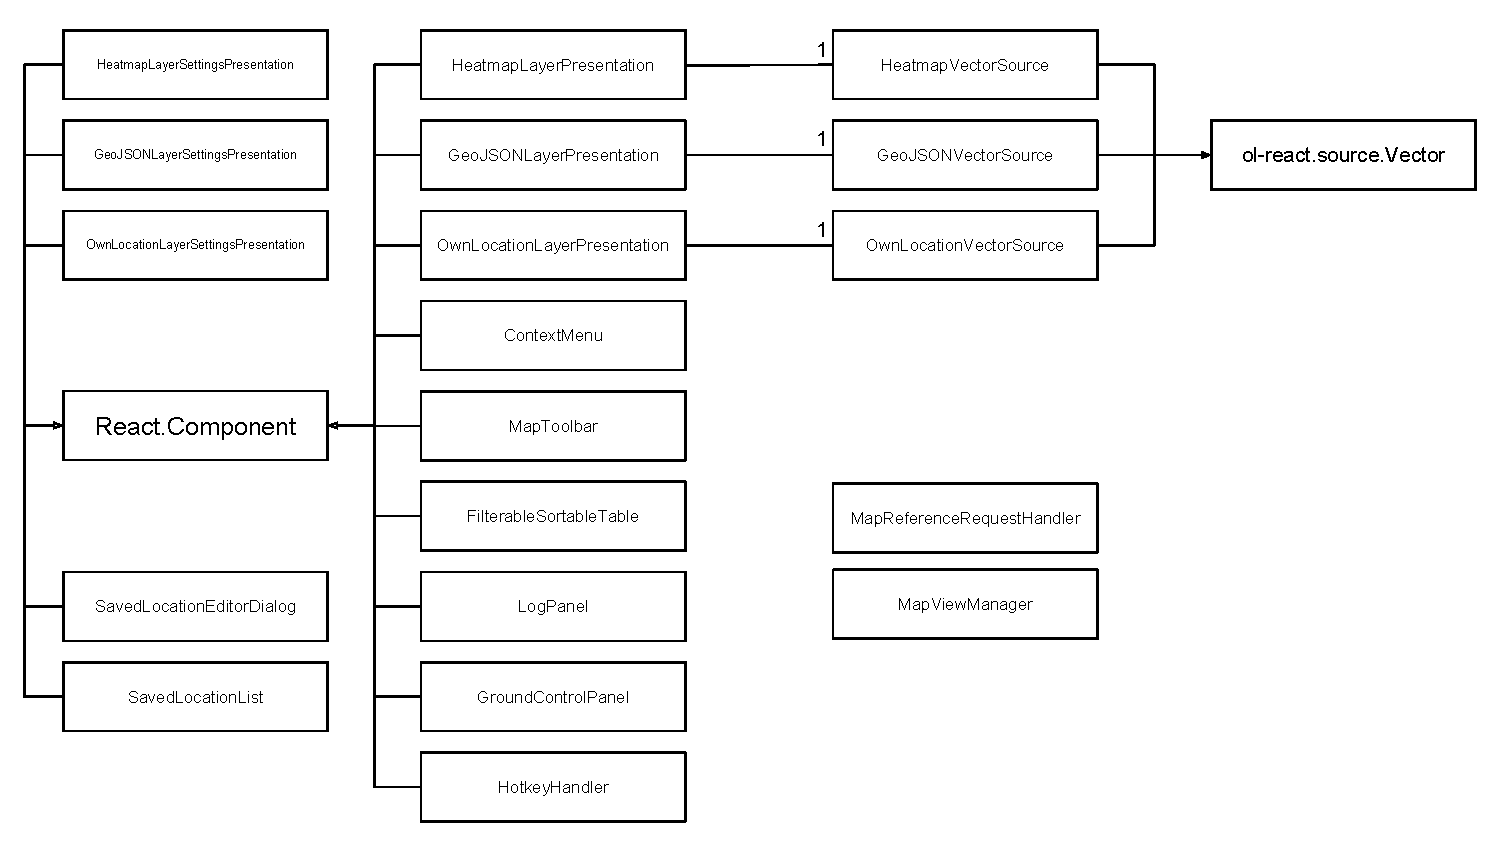
\includegraphics[width=\textwidth]{class_diagram.pdf}
  \caption{Osztálydiagram}
\end{figure}
